\documentclass[10pt, twocolumnjournal]{IEEEtran}
\usepackage{amsfonts, amsmath, latexsym, amssymb}
\usepackage{graphicx}
\usepackage{array}
\usepackage{soul, color, enumerate}
\usepackage{bm}
\usepackage{hyperref}
\usepackage{subfigure}

\title{Group Attribute Context-ware Password Guessing for Interactive Applications}
\author{C. Lu}

\begin{document}
	
\maketitle
	
\begin{abstract}	
\end{abstract}
	
\begin{IEEEkeywords}	
\end{IEEEkeywords}

\section{Introduction}
\label{sec:introduction}
%1. 背景
%2. 现有工作
%3. 存在的问题 
%4. 引出本文贡献(3个创新点列出)
%5. 文章的结构

	
\section{Related Works}
\label{sec:related}
%1. 列出前人工作(每个一段,5到6个)
%2. 总结 评价
\section{Group Attribute Password Guessing Scheme}
\subsection{Password Dataset Processing}
To train the password guessing model, we have collected a huge number of leaked and cracked password sets containing various group attributes. Table \ref{tb:password_set} illustrates some of the leaked password sets. Many of these passwords contain personal information about the owner, such as name, birthday, email, etc. In order to protect personal privacy, only the password was used in our experiments. We have selected five group attributes, corresponding to Game, Programmer, Marriage, Writing, Social. In order to represent these attributes, $1$-of-$N$ encoding has been used, that is, a five dimensional vector $\bm g_c$, where only the $c^{\mathrm{th}}$ dimension is one and the rest are zero. Each of the password set has been divided into three parts: a training set, a validation set and a test set. For the password in the test set we have used MD5 encryption so that the hashcat \ref{*} can be used to evaluate the efficiency of the generated password set by our model. Hashcat is an advanced password recovery tool.

As will be mentioned below, the main idea of the model is using the current password character to predict the next character. To achieve this, the trianing password was represented as matrices.  During training, we must specify the length of input sequence in the model, denoted by $T$ in this paper, which is a hyper parameter that needs to be set manually. Various sequence length has been tested and made comparisons, which will be shown in the section \ref{sec:evaluation}. Assume that the length of sequence is chosen as $4$, considering the password \emph{iloveyou}, the first input of the model is \emph{ilov}, and the corresponding label is \emph{love}. In the next round of training, the input becomes \emph{love}, and the label is changed to \emph{ovey}. In generation phase, for the same password \emph{iloveyou}, the first input character is \emph{i}, which can be represented by an $n$-dimensional vector, where $n$ refers to the size of  alphabet in password set. The model then learns that given the first character, the next character will be \emph{l}. The next time step, the model will loads in two characters, and learns given the sequence \emph{il}, the next character will be \emph{o}. This process is repeated until it generate the \emph{\textless eos\textgreater}, which refers to the end of a password.

\begin{table}
	\caption{Password sets for various group attributes}
	\label{tb:password_set}
	\centering
	\begin{tabular}{|c||c|c|c|}
	\hline
	\textbf{Password Set} & \textbf{Type} & \textbf{Leak Method}& \textbf{Total Number}  \\
	\hline
	Rock You & Game & SQL Injection & 32,603,388 \\ 
	\hline
	CSDN & Programmer & Hacking & 6,428,287 \\ 
	\hline   
	Flirtife.de & Marriage & Hacking & 115,589 \\ 
	\hline  
	Faithwriters & Writing & SQL Injection & 9,709 \\ 
	\hline 
	MySpace & Social & Phishing Attack & 41,545 \\ 
	\hline    
	\end{tabular}
\end{table}
	

\subsection{Model Architecture} 
In this work, we use recurrent neural networks which are a rich class of dynamic systems have been used for generate text in character level \cite{graves2013generating}. Recurrent neural networks can persists information entered into the system previously and then use it to predict or generate information. Because recurrent neural network can generate previously unseen informations (such as characters in password guessing), we will get some new passwords that don't appear in the training dataset. As shown in the next section, these new passwords will increase the guessing accuracy of dictionary attacks. We experimented with two different recurrent models in Section \ref{sec:evaluation}, one of which is Long Short-term Memory\cite{hochreiter1997long} and the other is Gated Recurrent Unit \cite{chung2014empirical}\cite{jozefowicz2015empirical}.

The password guessing model are organized into three major layers. The first layer is the embedding layer which is mainly used to encode the input characters into a vector. The next layer is the recurrent neural network, which is used to learn the hidden feature information in the password. At the same time, the encoded group attribute vector will be sent into this layer which is used to generate the passwords for specific user category. In the last layer, we use the fully connected layer and softmax activation function to output the probability distribution of the next character. Formally, the structure of the model can be expressed as follows.
\begin{align*}
	\bm e_t &= \bm f_{\mathrm{emb}}(\bm x_t) \\
	\bm h_t &= \bm f_{\mathrm{rnn}}(\bm e_t, \bm h_{t-1}) \\
	\bm o_t &= \bm f_{\mathrm{linear}}(\bm h_t, \bm g_c) \\
	\bm P(\mathcal A) &= \mathrm{softmax}(\bm o_t)
\end{align*}
where $\bm x_t$ denotes the input character at time step $t$, $\bm h_t$ denotes the hidden state of recurrent neural network, and $\bm f(\cdot)$ is the specific neural network function. $\bm g_c$ is the coding of group $c$. $\mathcal A$ denotes the alphabet has been used in password set which contains letters, digits and some special characters. $\bm P(\mathcal A)$ denotes the probability distribution of each character in alphabet. The brief structure of the model at time step $t$ is shown in Figure \ref{fig:sys_model}. We can use more than one recurrent layer. The number of layers is hyper parameter in our model. 
\begin{figure}
	\centering
	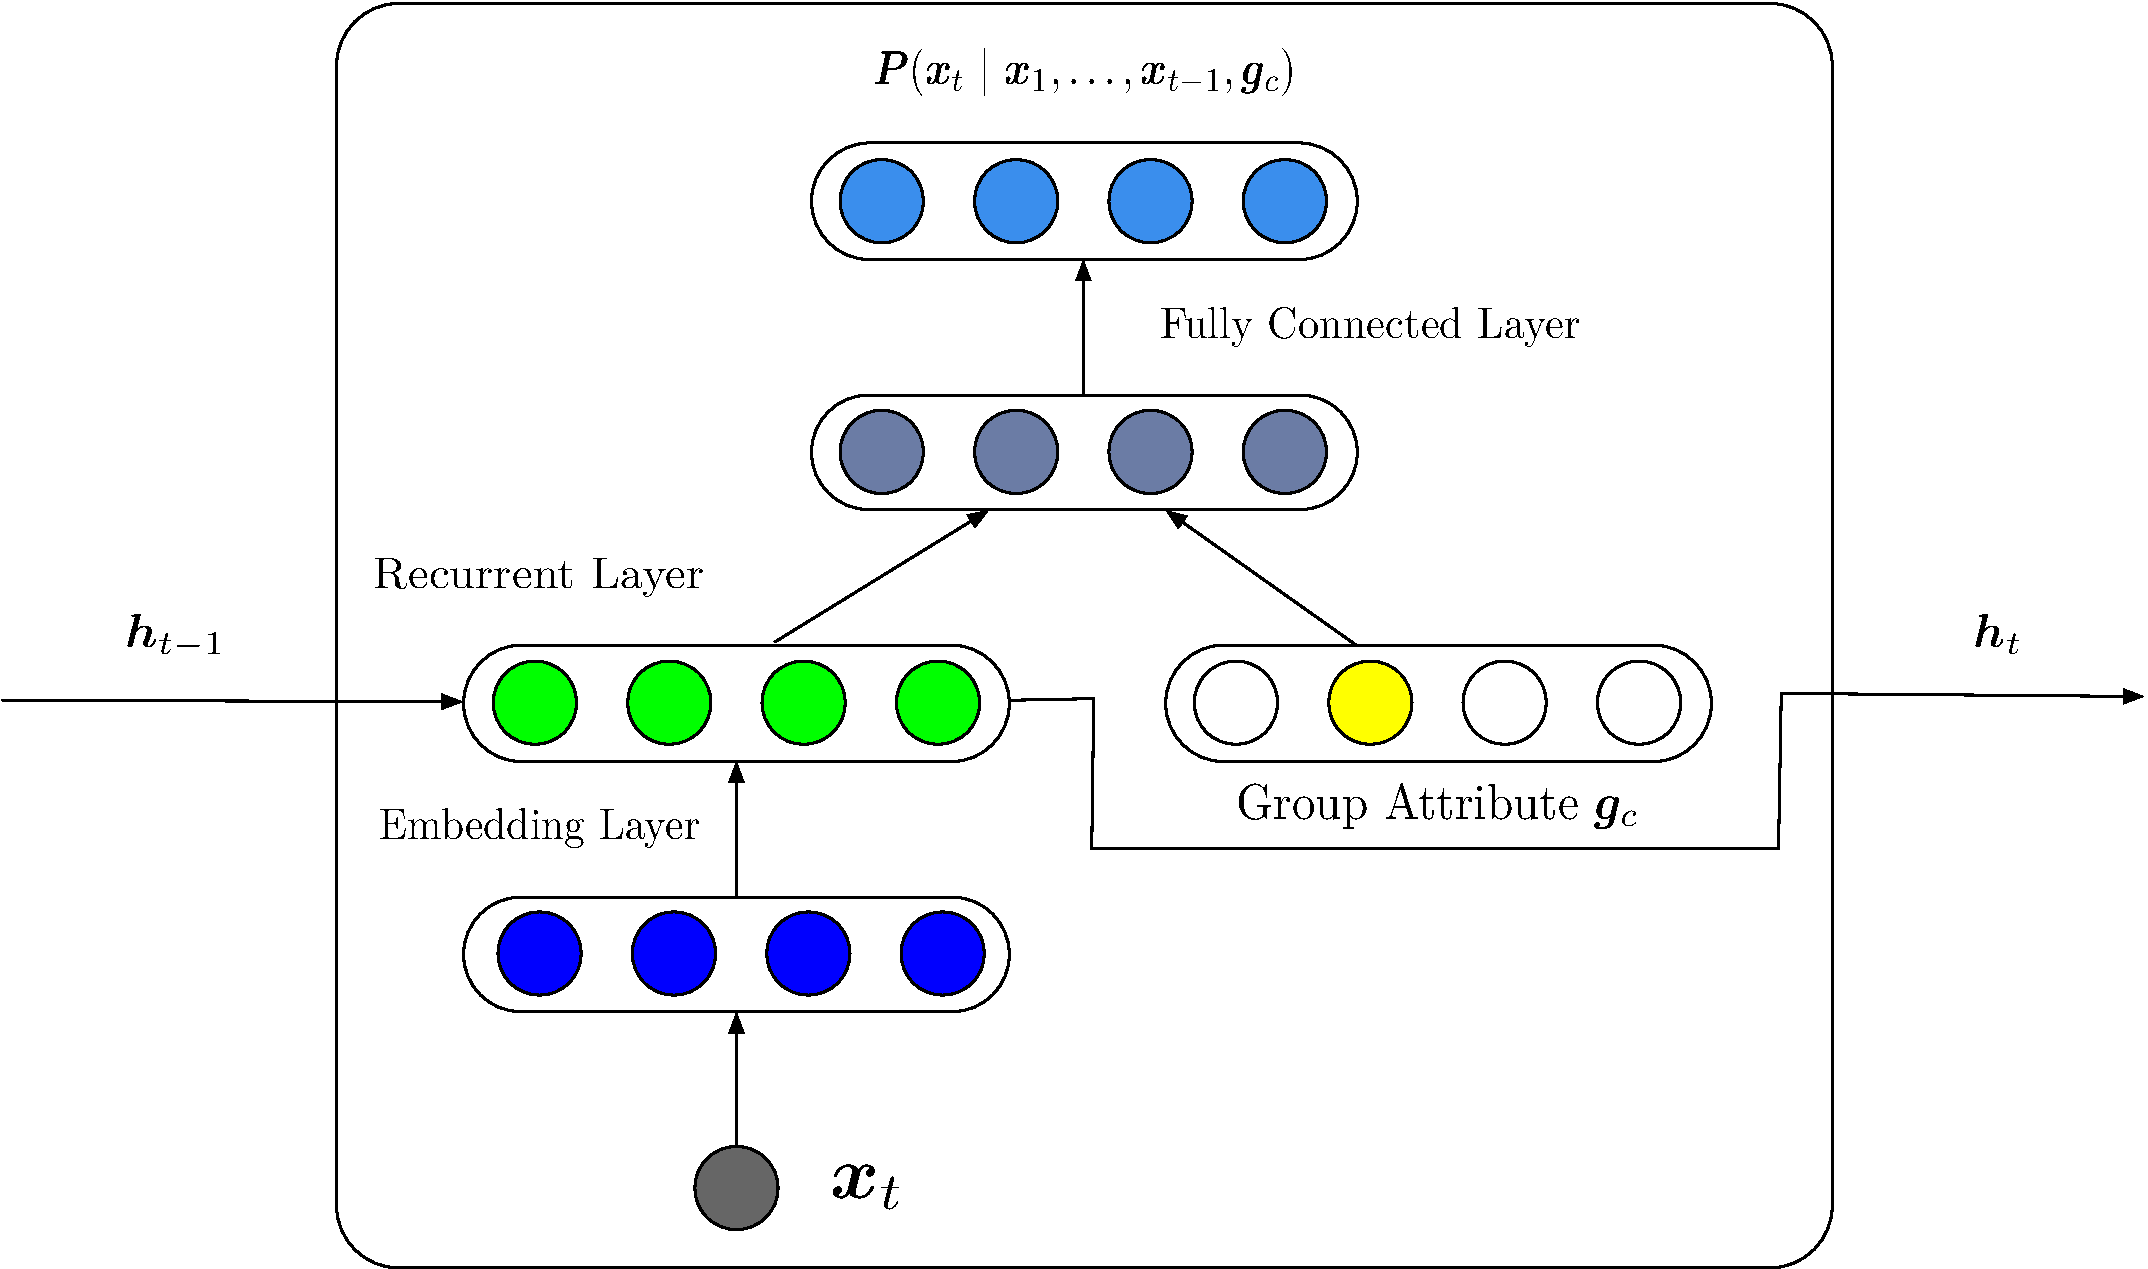
\includegraphics[width=8.5cm]{Model.pdf}
	\caption{ The structure of the model. It accepts previous hidden state $\bm h_{t-1}$ and character $\bm x_t$ at time step $t$, outputs the hidden state at next moment, and the probability of the next character.}
	\label{fig:sys_model}
\end{figure}


\subsection{Model Training}
To train the model, we used Tensorflow\cite{abadi2016tensorflow} , an open source deep learning library developed by Google. In the recurrent layer, there are three LSTM or GRU layers. The model was trained on two GTX1080Ti GPUs for about 18 hours. All of our code for the model was written in Python and the code can be found at github\footnote{https://github.com/luchu1993/Password-Generating-with-CharRNN}. There are many hyper parameters for training the model. We experimented with many options and eventually got a better configuration. The output dimension of the embedding layer is 64 and the dimension of recurrent layers are all 256, batch size of input in the model is 32. The details of the loss function are as follows. For each training password $\bm X$, the loss function $L(\cdot)$ at time step $t$ is that:
\begin{equation*}
	\begin{aligned}
		L(\bm x_t, \bm y_t) &= -\log \left(\frac{\exp\{ \bm o_t^{(\bm y_t)} \}}{\sum_{j}\exp\{\bm o_t^{(j)}\}}\right) \\ 
		&= -\bm o_t^{(\bm y_t)} + \log\left(\sum_{j}\exp\{\bm o_t^{(j)}\} \right)
	\end{aligned}
\end{equation*}
where $\bm x_t$ is the input and $\bm y_t$ is the label at time step $t$. $\bm o_t$ is the linear layer output. $\bm o_t^{(j)}$ denotes the $j^{\mathrm{th}}$ component in $\bm o_t$. The total loss $\mathcal L(\bm X)$ is the sum of the loss function values for all time steps.
\begin{equation*}
	\mathcal L(\bm X) = \sum_{t=1}^{T}L(\bm x_t, \bm y_t)
\end{equation*}


\subsection{Generating Passwords}
% 1. 介绍生成口令方法
%

\subsection{Probability-based Password Strength Measure}
The basic idea of the password strength measure is that the strength of a password is inversely proportional to the probability of its appearance. Given a group attribute $\bm g_c$, we can use the following equation to calculate the probability of a password $\bm X$:
\begin{equation*}
\begin{aligned}
	\bm P(\bm X\ |\ \bm g_c) & = \bm P(\bm x_1, \ldots, \bm x_T\ |\ \bm g_c)\\
	 & = \bm P(\bm x_1\ |\ \bm g_c)\prod_{t=2}^{T} \bm P(\bm x_t\ |\ \bm x_1\ldots\bm x_{t-1}, \bm g_c)
\end{aligned}
\end{equation*} 
where $T$ denotes the length of password. $\bm P(\bm x_1\ |\ \bm g_c)$ is a random multinomial distribution and $\bm P(\bm x_t\ |\ \bm x_1,\ldots, \bm x_{t-1}, \bm g_c )$ can be calculated by the model. When the probability of password $\bm X$ is calculated, its strength can be computed as follows.
\begin{equation*}
	\begin{aligned}
		\mathcal S(\bm X) = -\log \bm P(\bm X\ |\ \bm g_c) 
	\end{aligned}
\end{equation*}
where $\mathcal S$ denotes the password strength. Table \ref{tb:top-five} illustrates the five highest and lowest probability passwords in the training set.
\begin{table}
	\caption{Table of five worst/best passwords in training set}
	\label{tb:top-five}
	\centering
	\subtable[ Top-5 worst passwords] {
	\begin{tabular}{c|c}
		Password & Probability \\
		\hline
		12345678 & $0.002911$ \\
		iloveyou & $0.002900$ \\
		abcd1234 & $0.001365$ \\
		hello123 & $0.001355$ \\
		password & $0.001254$
	\end{tabular}
	}
	\qquad
	\subtable[Top-5 best passwords]
	{
	\begin{tabular} {c|c}
		Password & Probability \\
		\hline
		xyz2fgds3 & $2.450712\times 10^{-48}$ \\
		34dfxvdc & $2.565318\times 10^{-46}$ \\
		ypp88jtj & $ 9.192378\times 10^{-38}$ \\
		19@96fbqaz & $2.653402\times 10^{-36}$ \\
		g8m456gz & $6.811976\times 10^{-35}$
	\end{tabular}
	}
\end{table}

\section{Evaluation}
\label{sec:evaluation}
	 
\section{Conclusion}
	
	
\bibliographystyle{IEEEtran}
\nocite{*}\bibliography{reference}
	
\end{document}